\subsection{Symmetrische multiprocessing}

Traditioneel werd de computer gezien als een sequentiële machine omdat een processor telkens maar 1 instructie per keer kan uitvoeren en een instructie is een sequentie van bewerkingen.

Parallelle verwerkingen verbeteren de prestaties en verhogen soms de betrouwbaarheid. Twee benaderingen hiervan zijn: Symmetric MultiProcessors (SMP’s) en Clusters.


\subsubsection{Architectuur van SMP}

Flynn onderscheidde de volgende soorten computersystemen:

\begin{itemize}
\item SISD-stroom (Single Instruction Single Data) : één processor voert één instructiestroom uit voor het verwerken van gegevens die zijn opgeslagen in één geheugen.
\item SIMD-stroom (Single Instruction Multiple Data): één machine-instructie bestuurt de gelijktijdige uitvoering van een aantal verwerkingselementen in een vast patroon.
\item MISD-stroom (Multiple Instruction Single Data): dit is NOOIT geïmplementeerd geweest. Een reeks gegevens wordt verzonden naar een verzameling processors, die elk een andere instructiereeks uitvoeren.
\item MIMD-stroom (Multiple Instruction Multiple Data): een verzameling processors voert tegelijk verschillende instructiereeksen uit met verschillende gegevensverzamelingen.
\end{itemize}

\newpage

Classificatie van multiprocessors met gedeeld geheugen (zie onderstaande afbeelding)

\begin{comment}

\begin{figure}[htp]
    \centering
            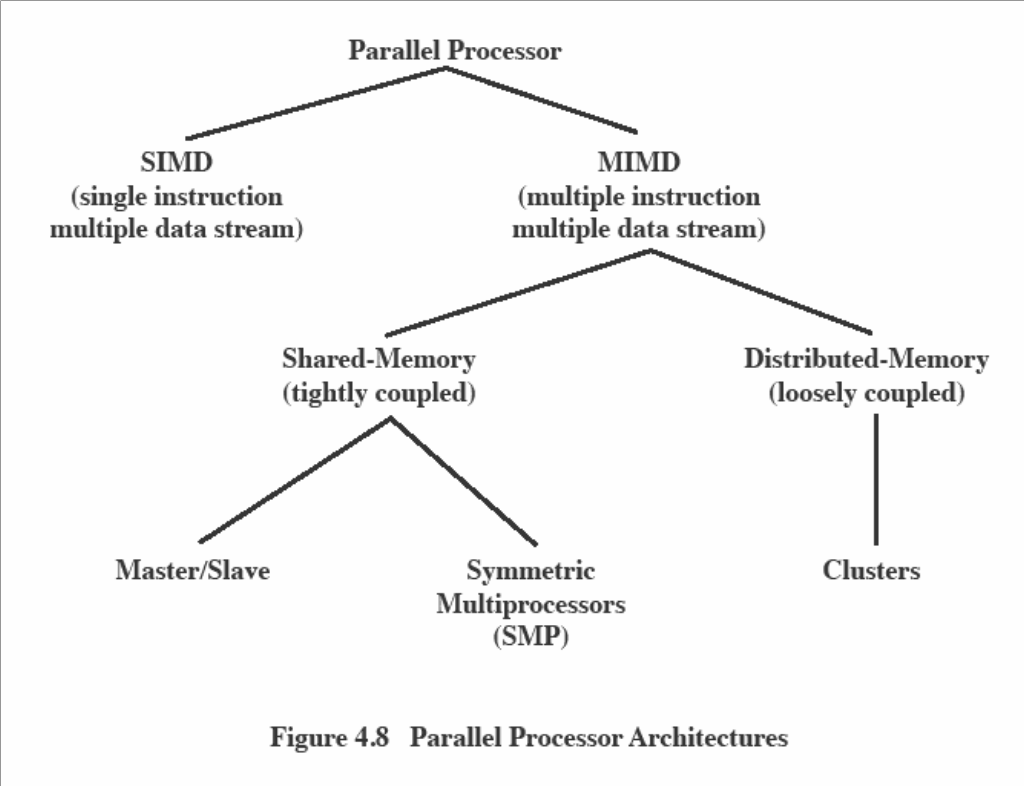
\includegraphics[width=4in]{img/classificatiemultiprocessors.png}
        \caption{Classificatie van multiprocessors met gedeeld geheugen}
    \label{fig:Classificatie van multiprocessors met gedeeld geheugen}
\end{figure}

\end{comment}

%To prevent floating at all we must not use the figure environment. The caption package gives a way to get all the other features. It provides the command \captionof that takes a counter (figure or table) as argument and of course the caption text, for example:

\begin{center}
            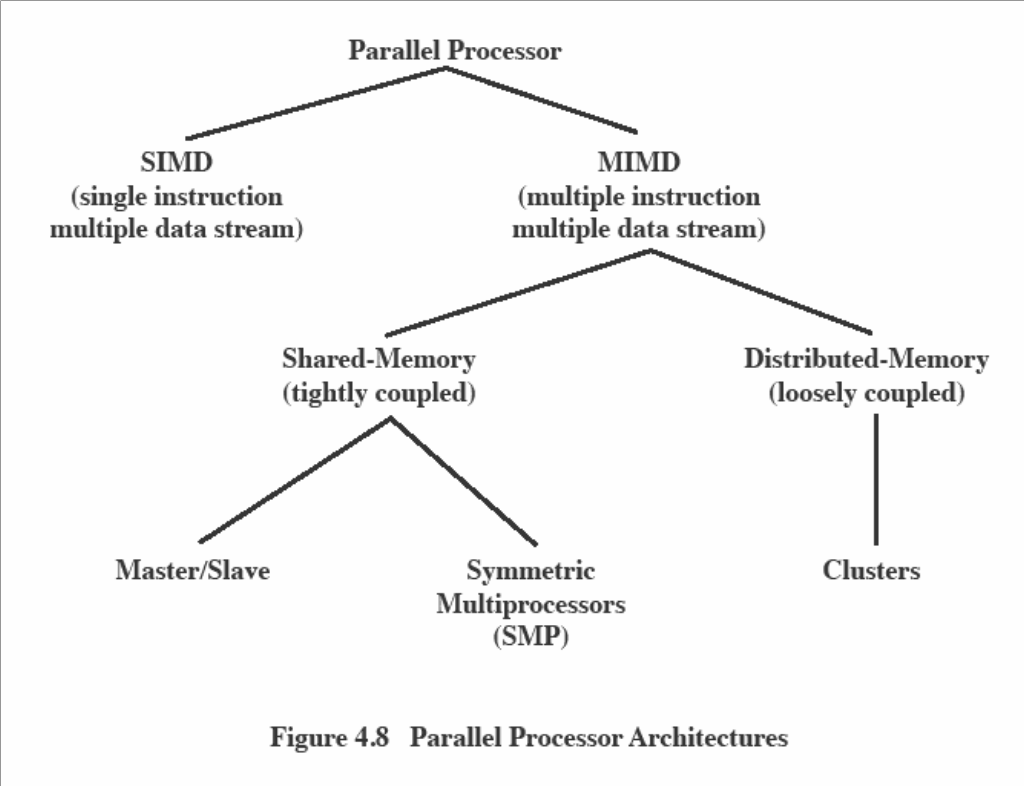
\includegraphics[width=4in]{img/classificatiemultiprocessors.png}
    \captionof{figure}{Classificatie van multiprocessors met gedeeld geheugen}\label{fig:Classificatie van multiprocessors met gedeeld geheugen}%
\end{center}

Bij Symmetrische multiprocessing kan de kernel worden uitgevoerd op elke processor en meestal verzorgt elke processor zelf de scheduling van de verzameling aanwezige processen of threads.

\newpage

\subsubsection{Organisatie van een typische Symmetrische Multiprocessing organisatie (zie onderstaande afbeelding)}
\begin{figure}[htp]
    \centering
            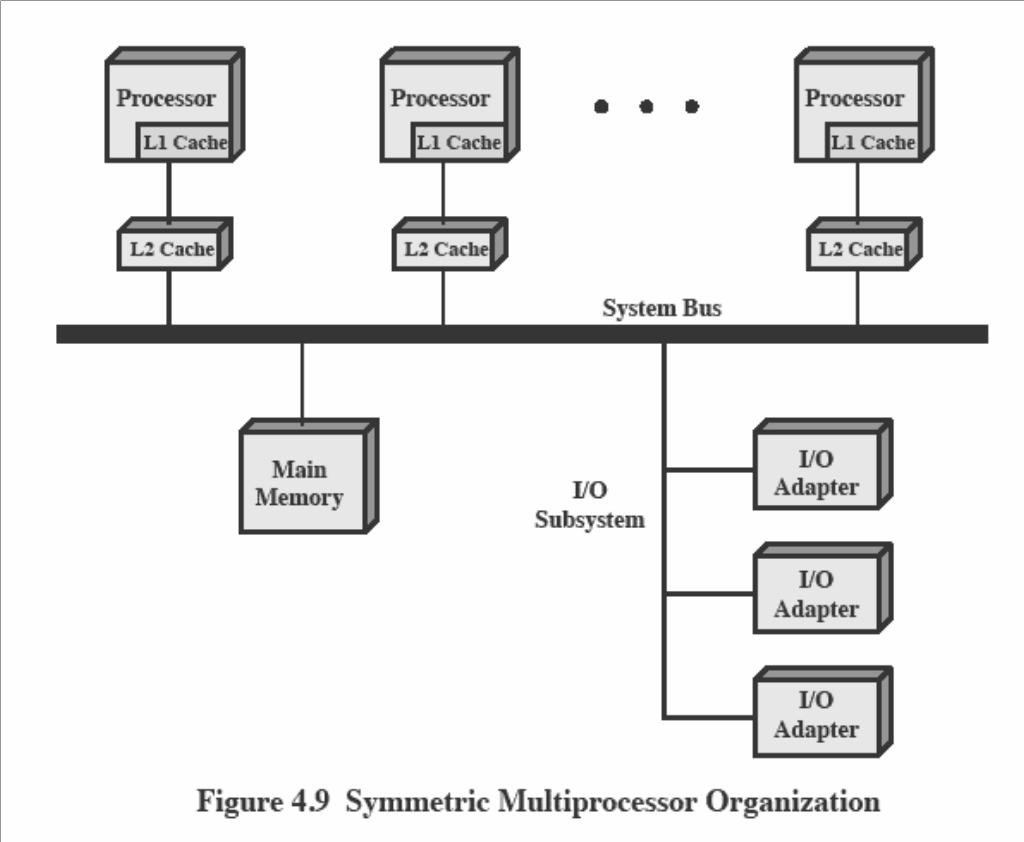
\includegraphics[width=4in]{img/organisatiesymmulti.png}
        \caption{Organisatie van een typische Symmetrische Multiprocessing organisatie}
    \label{fig:Organisatie van een typische Symmetrische Multiprocessing organisatie}
\end{figure}


\subsubsection{Ontwerpen van besturingssystemen voor SMP}

\textbf{De belangrijkste aandachtspunten voor het ontwerpen van een besturingssysteem voor SMP zijn:}

\begin{itemize}
\item Gelijktijdig samenwerkende processen of threads. Kernelroutines moeten herintredend zijn om verschillende processors de mogelijkheid te bieden dezelfde kernelcode gelijktijdig uit te voeren. De kerneltabellen en beheerstructuren moeten goed worden beheerd om deadlocks of ongeldige bewerkingen te voorkomen.
\item Scheduling. Het schedulen kan worden uitgevoerd door elke processor, dus conflicten moeten worden vermeden.
\item Synchronisatie. Bij meerdere actieve processen die toegang kunnen hebben tot gedeelde adresruimten of gedeelde I/O-bronnen, moet worden gezorgd voor een effectieve synchronisatie, wat zorgt voor een wederzijdse uitsluiting en het ordenen van gebeurtenissen.
\item Geheugenbeheer. Het geheugenbeheer van een multiprocessor moet alle mogelijkheden bieden van machines met één processor. Daarnaast moet het besturingssysteem de parallelliteit benutten die beschikbaar is in de hardware, zoals geheugens met meerdere poorten, voor het bereiken van optimale prestaties.
\item Betrouwbaarheid en fouttolerantie. Het besturingssysteem moet bij processorstoringen voorzien in een geleidelijke en nette noodprocedure. De scheduler en andere delen van het besturingssysteem moeten een verlies van een processor herkennen en de tabellen voor het beheer daaraan aanpassen.
\end{itemize}